\chapter{Supersymmetry and the Standard Model}
\label{ch:SUSY}

The fundamental theory of particle physics, known as the Standard Model (SM) can predict precise interactions between the fundamental particles in our universe. With these predictions we are able to confirm processes, but there are some aspects of the universe that have not yet been explained. In this chapter, we will analyze the Standard model and the respective models that cannot be explained.

\section{The Standard Model}
\label{sec:SM}

After decades of theoretical and experimental research the SM has been developed into a theory that explains the Electromagnetic (EM), Strong, and Weak force. The SM has not yet been able to include Gravity into the theory. With the robust theoretical and experimental methods used in the SM, we have discovered new elementary particles and predicted others. 

\section{The Fundamental Particles}

 All the matter can be explained by three kinds of elementary particles: leptons, quarks, and gauge bosons. Each of these can be distinguished by various respective properties. The leptons and quarks are fermions which are particles that have half-integer spin. The leptons are particles that only interact with the EM force, while quarks interact with the EM and Strong force. The gauge bosons are the force carries for each respective force and have integer spin. 
 
 There are three generations of leptons and quarks which are differentiated by a charge $\pm e$, the charge of an electron. The leptons have three different charged particle: electron $(e)$, muon $(\mu)$, and tau $(\tau)$. With each charged particle having a corresponding neutrino $(\nu)$ of the same flavour, see fig \ref{SMParticles}. The quarks are also separated into three generations of doublets, the down-type $(-\frac{1}{3}e)$: down $(d)$, strange $(s)$, and bottom $(b)$ and up-type $(\frac{2}{3}e)$: up $(u)$, charm $(c)$, and top $(t)$, see fig \ref{SMParticles}. Each of the quarks has a color associated with it with is analogous to an electric charge, except there are three colors charges: red, blue, and green.  

\begin{figure}
 	\centering
	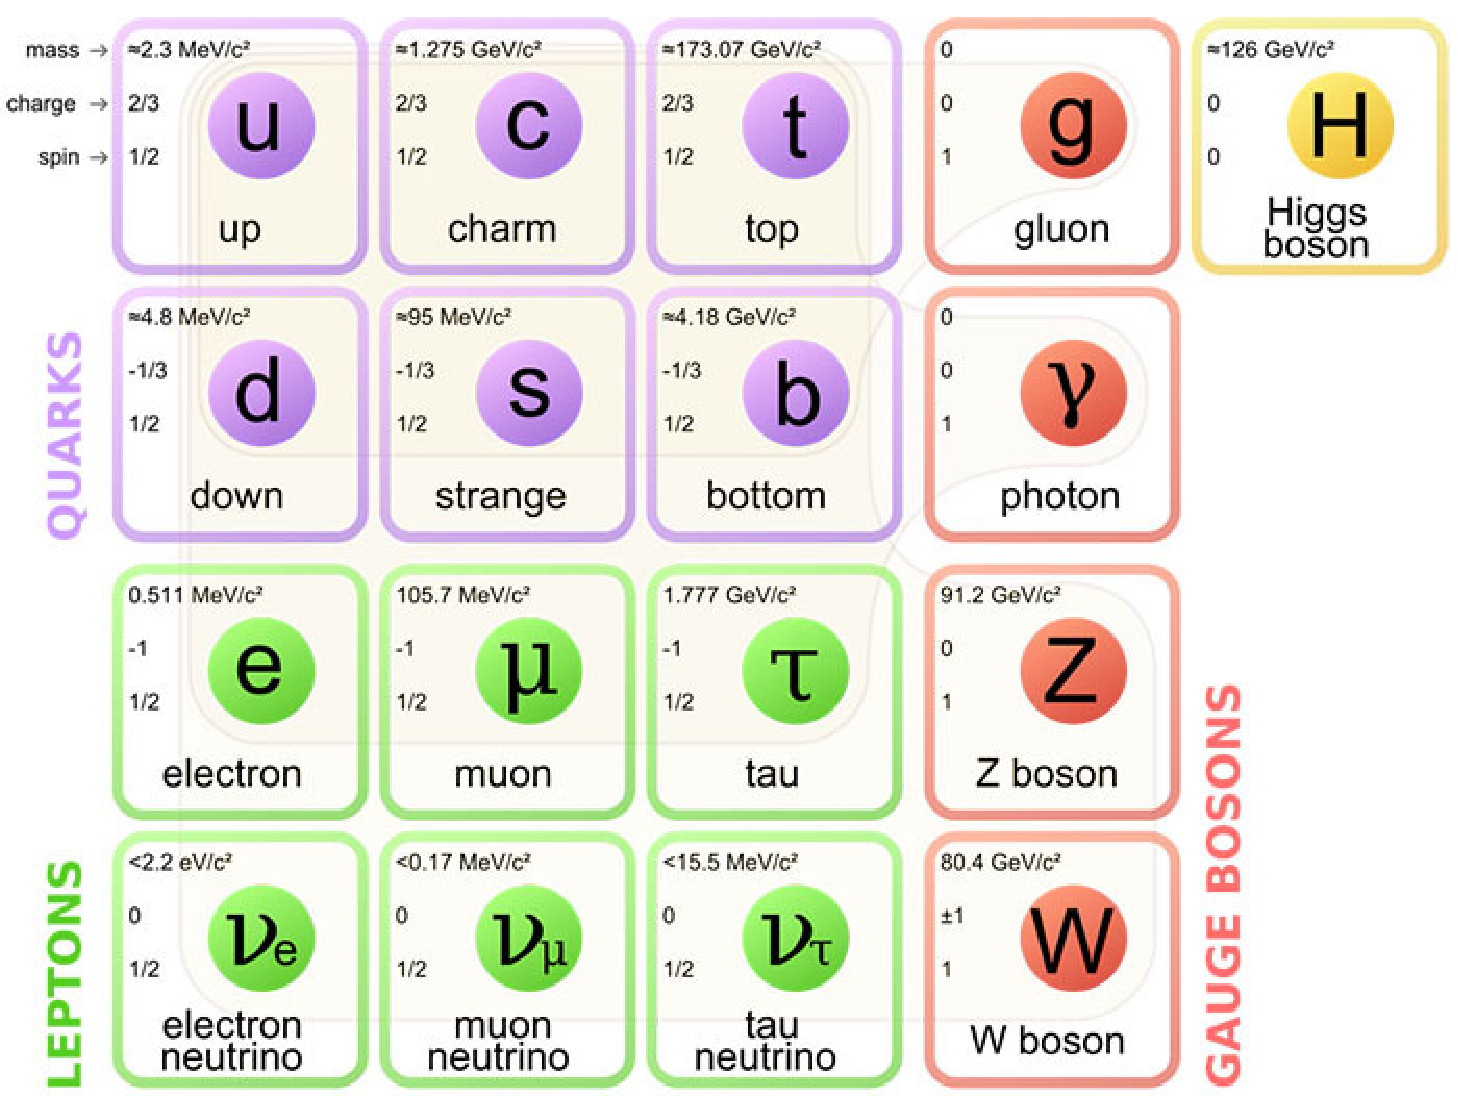
\includegraphics[width=0.75\textwidth]{StandardModel.pdf}
 	\caption{The fundamental particles of the Standard Model. There are three generations of quarks and leptons. Along with the five bosons, where four of them relate to the interactions of the three forces included in the SM: Electromagnetism, the Weak force, and the Strong force and the final being the Higgs boson which give mass to particles. }
 	\label{SMParticles} 
\end{figure}
 
 \section{Quantum Field Theory}
 \label{QFT}
 
 The interactions of all of these particles are described by the interactions of quantized fields. These fields become operators that describe the creation and annihilation of particles. Each of the fields of the SM have a corresponding boson, see fig. \ref{SMParticles}. The most well known field being the Electromagnetic (EM) field and its interactions. 
 
 First, we start with the assumption that the wave function $\psi(x)$ should transform as,
 
 \begin{equation}\label{U1gauge}
 \psi(x)\rightarrow e^{i\alpha(x)}\psi(x),
 \end{equation}
 
 where $\alpha(x)$ has an arbitrary dependence on space and time. If one were to include this into the Dirac equation you would find that it is not invariant under such a local phase transformation. To include an invariace of the field, we must include a derivative, $D_\mu$, that is covariant under phase transformations,
 
 \begin{equation}\label{QEDCovariantD}
 D_\mu\equiv\partial_\mu-ieA_\mu.
 \end{equation}
 
 The covariant derivative must include the vector field $A_\mu$ which must also transform as,
  
 \begin{equation}\label{PhotonField}
 A_\mu\rightarrow A_\mu+\frac{1}{e}\partial_\mu\alpha.
 \end{equation}
 
 So after requiring that there be a local gauge transformation, we were forced to introduce a vector field $A_\mu$, called the guage field, which couples to Dirac particles in the same way as the photon field. We will think of this new field as the real photon field, which means we need to add a kinematic energy portion to the lagrangian. This kinematic term will be invariant under Eqn. \ref{PhotonField} which leads us to final final representation of the QED lagrangian which can be written down concisely as, 
 
 \begin{equation}\label{LagrangianQED}
\mathcal{L}_{QED}=\overline{\psi}(i\gamma^\mu\partial_\mu-m)\psi+e\overline{\psi}\gamma^{\mu}A_{\mu}\psi-\frac{1}{4}F^{\mu\nu}F_{\mu\nu},
 \end{equation}

where $\gamma^\mu$ are invariant tensors, $\partial_\mu$ is the partial derivative, $m$ is the mass of the particle, $\psi$ is the wave function of the particle, $A_{\mu}$ is the EM field operator, and $F^{\mu\nu}$ is the EM field tensor. Each of the parts of this equation are lorentz invariant which allows this to be true in all reference frames. This lagrangian describes the interactions of a particle and the EM field moving through spacetime. 

After this we will transition from the description of the $U(1)$ EM field to the $SU(3)$ QCD field and the transformation of quark fields. A free moving quark is described by,

\begin{equation}\label{LagrangianQCDVacuum}
\mathcal{L}_{QCD}^{vac}=\overrightarrow{q}_j(i\gamma^\mu\partial\mu-m)q_j,
\end{equation}

where $q_1, q_2,$ and $q_3$ are the three color fields. From this we want the we want to require that the field is again invariant under another local phase transformation such as,

\begin{equation}
q(x)\rightarrow Uq(x)\equiv e^{i\alpha_a(x)T_a}q(x),
\end{equation}

where $U$ is a $3\times3$ unitary matix, $T_a$ with $a=1,...,8$ are a set of linearly independent traceless $3\times3$ matrices, and $\alpha_a$ are the group parameters. Since the generators $T_a$ do not necessarily commute with each other, we can see that it is indeed non-Abelian and the commutator of can be represented as,

\begin{equation}
[T_a, T_b]=if_{abc}T_c,
\end{equation}

where $f_{abc}$ are constants. 

We need to impose $SU(3)$ local gauge invariance on Eqn. \ref{LagrangianQCDVacuum}, we allow for the following phase transformations,

\begin{equation}
\begin{split}
& q(x)\rightarrow[1+i\alpha_a(x)T_a]q(x), \\
& \partial_\mu q\rightarrow(1+i\alpha_aT_a)\partial_\mu q+iT_aq\partial_\mu\alpha_a.
\end{split}
\end{equation}

From this is seems straight forward that we can proceed in exactly the same manner as QED, which is to add

\begin{equation}
G_\mu^a\rightarrow G_\mu^a-\frac{1}{g}\partial_\mu\alpha_a, 
\end{equation}

and a covariant derivative

\begin{equation}
D_\mu=\partial_\mu+igT_aG_\mu^a.
\end{equation}

This will give us a similar lagrangian to the QED one derived above, but this is not sufficient for a non-Abelian gauge transformation and is does not produce a gauge-invariant Lagrangian. One final transformation is required for the $G_\mu^a$ fields to achieve gauge invariance, 

\begin{equation}\label{QCDGaugeTransform}
G_\mu^a\rightarrow G_\mu^a-\frac{1}{g}\partial_\mu\alpha_a-f_{abc}\alpha_b G_\mu^c,
\end{equation}

This finally give us a gauge invariant kinetic energy term for all of the $G_\mu^a$ fields and thus we can write the QCD interactions as,

\begin{equation}\label{LagrangianQCD}
\mathcal{L}_{QCD}=\overline{q}(i\gamma^\mu\partial_\mu-m)q-g(\overline{q}\gamma^\mu T_a q)G^a_\mu-\frac{1}{4}G^a_{\mu\nu}G_a^{\mu\nu}.
\end{equation}

From all of this we seem to be missing a vital part of the SM, specifically a theory for the Weakly interacting processes which is mediated by the massive bosons, $W$ and $Z$ from fig. \ref{SMParticles}. This requires the Higgs Mechanism.

\section{The Higgs Mechanism}

We are interested in the spontaneous symmetry breaking of a local $SU(2)$ gauge symmetry. We are interested in the following $SU(2)$ Lagrangian,

\begin{equation}\label{HiggsLagrangian}
\mathcal{L}=(\partial_\mu\phi)^\dagger(\partial^\mu\phi)-\mu^2\phi^\dagger\phi-\lambda(\phi^\dagger\phi)^2,
\end{equation}

with $\phi$ being a $SU(2)$ doublet of complex scalar fields

\begin{equation}
\phi=\frac{1}{2}
\begin{bmatrix}
\phi_1+i\phi_2 \\
\phi_3+i\phi_4
\end{bmatrix}
\end{equation} 

and is invariant under global the $SU(2)$ phase transformations $\phi\rightarrow e^{i\alpha_a\tau_a/2}\phi$. To allow for local invariance, we first allow for a covariant derivative

\begin{equation}
D_\mu=\partial_\mu+ig\frac{\tau_a}{2}W_\mu^a,
\end{equation}

where we now have three gauge fields, $W_\mu^a$ with $a=1,2,3$. If we assume an infanitesimal gauge transformation for the $SU(2)$ doublet $\phi(x)\rightarrow\phi'(x)=(1 +i\boldsymbol{\alpha}(x)\cdot\boldsymbol{\tau}/2)\phi(x)$, then the gauge fields will transform as

\begin{equation}\label{HiggVectorTransform}
\boldsymbol{W}_\mu\rightarrow\boldsymbol{W}_\mu-\frac{1}{g}\partial_\mu\boldsymbol{\alpha}-\boldsymbol{\alpha}\times\boldsymbol{W}_\mu,
\end{equation}

you can see that Eqn. \ref{HiggVectorTransform} is just the compact vector transform of Eqn. \ref{QCDGaugeTransform} where we have replaced the QCD gauge field with the three gauge fields $W_\mu^a$. If we include these locally invariant transformations into the above $SU(2)$ Lagrangian we get

\begin{equation}\label{HiggsInvariantL}
\mathcal{L}=(\partial_\mu\phi+ig\frac{1}{2}\boldsymbol{\tau}\cdot\boldsymbol{W}_\mu\phi)^\dagger(\partial^\mu\phi+ig\frac{1}{2}\boldsymbol{\tau}\cdot\boldsymbol{W}^\mu\phi)-\mu^2\phi^\dagger\phi+\lambda(\phi^\dagger\phi)^2-\frac{1}{4}\boldsymbol{W}_{\mu\nu}\cdot\boldsymbol{W}^{\mu\nu},
\end{equation}

where the inclusion of the gauge field kinetic term has been included at the end. The most interesting regions of this lagrangian is when $\mu^2<0$ and $\lambda>0$, where the potential has a minimum at $\phi^\dagger\phi=-\frac{\mu^2}{2\lambda}$. With this we will expand the potential around the minimum and require that

\begin{equation}
\phi_1=\phi_2=\phi_4=0, \phi_3^2=-\frac{\mu^2}{2\lambda}\equiv v^2.
\end{equation}

This is the spontaneous symmetry breaking of the $SU(2)$ symmetry, because of this we are able to substitute an expansion for the field

\begin{equation}
\phi=\sqrt{\frac{1}{2}}
\begin{bmatrix}
0 \\
v+h(x)
\end{bmatrix}
\end{equation}

With this specific transformation of the $SU(2)$ doublet and the simplification of Eqn. \ref{HiggsInvariantL}, the only remaining field is $h(x)$ which is refered to as the Higgs field. This is what is known as the Higgs Mechanism. 

We want to include the methods of the Higgs Mechanism into the weak isospin and weak hypercharge,$SU(2)_L\times U(1)_Y$, transformations of electoweak interactions. First, we need to include the coupling of the weak currents $\boldsymbol{J}_\mu$ and the gauge field $\boldsymbol{W}^\mu$ such that,

\begin{equation}
-ig\boldsymbol{J}_\mu\cdot\boldsymbol{W}^\mu=-ig\overline{\chi}_L\gamma_\mu\boldsymbol{T}\cdot\boldsymbol{W}^\mu\chi_L
\end{equation}

which is the basic interaction for the $SU(2)_L$ symmetry. Then, we also need to include the weak hypercharge current with the fourth vector boson $B^\mu$,

\begin{equation}
-i\frac{g'}{2}j_\mu^YB^\mu=-ig'\overline{\psi}\gamma_\mu\frac{Y}{2}\psi B^\mu, 
\end{equation}

here the operators $\boldsymbol{T}$ and $Y$ are generators for the $SU(2)_L$ and $U(1)_Y$ gauge transformations, respectively. Now we combine the two symmetries with the transformations of the left and right hand components of $\psi$ as

\begin{equation}
\begin{split}
\chi_L\rightarrow\chi'_L&=e^{i\boldsymbol{\alpha(x)\cdot T+i\beta(x)Y}}\chi_L, \\
\psi_R\rightarrow\psi'_R&=e^{i\beta(x)Y}\psi_R
\end{split}
\end{equation}

from this we can write down the contributions of the two gauge fields $\boldsymbol{W}_\mu^3$ and $B_\mu$ and the mising angle $\theta_W$ to find the interactions of the two neutral currents. The physical fields are thus,

\begin{equation}
-igJ_\mu^3W^{3\mu}-i\frac{g'}{2}j_\mu^YB^\mu=-iej_\mu^{em}\boldsymbol{A}^\mu-\frac{ie}{sin\theta_Wcos\theta_W}[J_\mu^3-sin^2\theta_Wj_\mu^{em}]Z^\mu.
\end{equation}

From this we can write down the Electroweak Lagrangian, for any fermion that interacts with the field. Moreover, we can formulate the Higgs mechanism, such that we can calculate the theoretical masses of the gauge bosons and fermions, such as, 

\begin{equation}
\begin{split}
& M_W=\frac{1}{2}vg \\
& M_Z=\frac{1}{2}v\sqrt{g^2+g'^2},
\end{split}
\end{equation}

but these masses cannot be predicted since the depend on the values from the chosen Higgs field. 

\subsection{The Standard Model Lagrangian}

With the inclusion of the Higgs mechanism and the formulation of a local gauge invariant Lagrangian for the Electroweak and QCD fields, we have the complete SM Lagrangian as,

\begin{equation}\label{SMLagrangian}
\begin{split}
\mathcal{L}=&-\frac{1}{4}\boldsymbol{W}_{\mu\nu}\boldsymbol{W}^{\mu\nu}-\frac{1}{4}B_{\mu\nu}B^{\mu\nu} \\
&+\overline{L}\gamma^\mu(i\partial_\mu-g\frac{1}{2}\boldsymbol{\tau}\cdot\boldsymbol{W}_\mu-g'\frac{Y}{2}B_\mu)L \\
&+\overline{R}\gamma^\mu(i\partial_\mu-g'\frac{Y}{2}B_\mu)R \\
&+\lvert(i\partial_\mu-g\frac{1}{2}\boldsymbol{\tau}\cdot\boldsymbol{W}_\mu-g'\frac{Y}{2}B_\mu)\phi\lvert^2-V(\phi) \\
&-(G_1\overline{L}\phi R+G_2\overline{L}\phi_cR+\text{hermitian conjugate}),
\end{split}
\end{equation}

where the first terms are the kinetic energies and self-interations of the $W^\pm,Z, \text{and} \gamma$ bosons, the second and third terms are the kinetic energies and interactions of the leptons and quarks with the $W^\pm,Z, \text{and} \gamma$ bosons where $L$ is a left-handed fermion doublet and $R$ is a right-handed fermion singlet. This is because the weak force only couples to left-handed fermions. The fourth term is the $W^\pm,Z,\gamma$ and Higgs masses and couplings. The final term is the lepton and quark masses and couplings to the Higgs field.  

\section{Fundamental Problems in the Standard Model}
\label{sec:SMIssues}

The SM has been able to accurately and precisely describe many facits of the universe. Whether is comes to predicting the existance of a sixth quark or the confirmation of the $g - 2$ of the muon to 9 orders of magnitude. Unfortunately, there is some evidence of matter or interactions that cannot be described such as dark matter, the Hierarch problem, or a possible grand unified theory. Let's look into each of these further.

\subsection{Dark Matter}
The amount of visible matter in the universe does not explain all of the measurable matter. This has most notibly been seen in the radial velocity of galaxies. In a universe which is solely made up of visible matter, matter that interacts with light, the radial velocity of stars should decrease the further away it is from the galactic nuclei. Though measurements show the velocity becoming constant as a function of radius. To reproduce these features in models, the mass of the galaxy must be significantly more that what is seen. This implies some unseen dark matter, that still interacts with the gravitational field but not with the EM field.There is currently no such particle that has these properties in the SM.

\begin{figure}
 	\centering
	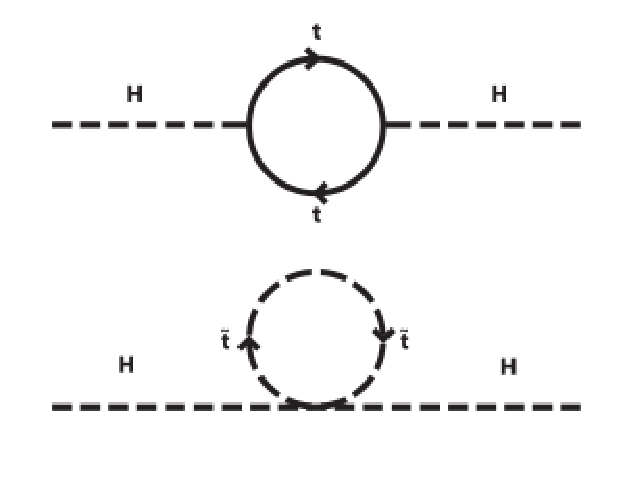
\includegraphics[width=0.5\textwidth]{Hierarchy.pdf}
 	\caption{The loop corrections to the Higgs boson interacting with a top quark and its superpartner the top squark. This is only the NLO corrections to the Higgs boson mass.}
 	\label{HiggsMass} 
\end{figure}

\subsection{Hierarchy Problem} 
The higgs boson is a beautiful solution to electroweak symmetry breaking and gives a method for particles to aqcuire mass and was discovery to have a measured mass, $m_{H}=125.15$ GeV. This value though is not predictable with the SM and leads to some inconsistencies when you include loop corrections. Since the higgs is strongly coupled to particles with large masses, the dominant loop correction will be due to interactions with $t$. These higher order loop corrections to the higgs mass, $m_H^2$, caused by the fermionic $t$ loop, see fig \ref{HiggsMass}, is

\begin{equation} \label{HiggsDivergence}
\Delta m_{H}^{2}=-\frac{|\lambda_{f}|^{2}}{8\pi^{2}}\Lambda_{UV}^{2}+\cdot\cdot\cdot,
\end{equation}

where $\lambda_f$ is the vertex factor for the respective fermion and $\Lambda_{UV}$ is the ultraviolet momentum cutoff. The higgs boson loop corrections are highly dependent on all virtual and real particles that couple to the higgs field. From this, we can see the corrections from Eqn. \ref{HiggsDivergence} for each fermion in the SM will cause a large divergence. The quadratic divergence of the higgs mass is only renormalizable with a fine tuning of the parameters $\lambda_f$ and $\Lambda_{UV}$. This means the only way for the SM to reconcile this unfortunate fact is to have a relatively luck cancellation of very large numbers of order $10^{32}$ with equally small numbers. If we look at the contribution with the addition a scalar partner to the fermion the higgs loop corrections reduce to,

\begin{equation}
\Delta m_{H}^{2}=\frac{\lambda_{S}}{16\pi^{2}}[\Lambda_{UV}^{2} - 2m_{S}^{2}ln(\Lambda_{UV}/m_{S})+\cdot\cdot\cdot].
\label{HiggsRenormalization}
\end{equation}

With the introduction of a scalar partner to the $t$, there is a logarithmic divergence to the higgs boson mass and can be renormalized through the normal methods.

\subsection{Grand Unified Theory}

The SM is able to accurately describe three of the fundamental sources at typical energy scales, 1 to $10^{4}$ GeV, but idealy the forces would be able to merge into a single force at high energies. This has not been directly observed, but many theories, such as SUSY, predict its existance %\cite{martin_supersymmetry_1997}.

\begin{figure}
 	\centering
	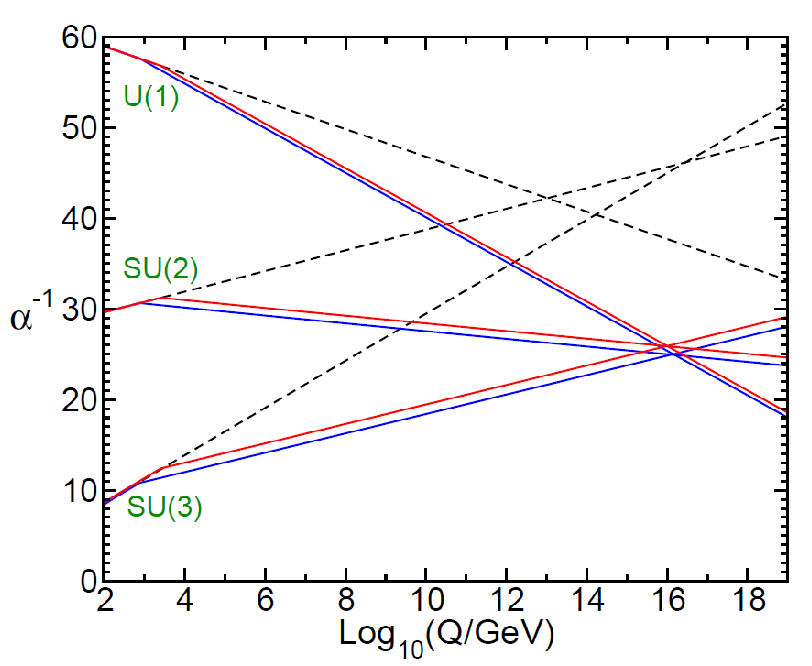
\includegraphics[width=0.5\textwidth]{GUTRenormalization.png}
 	\caption{The energy dependence of the inverse gauge couple of each force in the SM (dashed line) and the MSSM (solid lines). The MSSM gives two thresholds for the sparticle mass 750 GeV and 2.5 TeV.}
 	\label{GUT} 
\end{figure}


\section{Superpartners}
\label{sec:superpartners}

With no additional information to hint at physics at scale about the TeV range, it seems that we need a new framework for physics at the reduced Planck scale $M_{P}=(8\pi G_{Newton})^{-1/2}=2.4\times10^{18}$ GeV, which is the scale at which quantum gravitational effects become important. The ratio of $M_p/M_W$ is a strong hint that there is more physics at scales beyond the SM. The Higgs field will become extremely important at these higher energy scales

Supersymmetry is broken into Chiral supermultiplets, which are fields that contain equal numbers of fermions and bosons. Each of these supermultiplets can transform and interact with each other. 

\subsection{Chirality}
\label{subsec:chiral}

Equal numbers of fermions and bosons. How does the spin change? 

\section{Minimal Supersymetric Standard Model}
\label{sec:MSSM}

Soft supersymetry breaking. 

\subsection{R Parity}
\label{subsec:rparity}

New conserved parameter known as R parity. With this is allows for a stable particle that is a dark matter candidate. Other consequences.

\section{Mass Spectrums}

Higgs boson corrections. spectrum of squarks. 






